\item {\bf Experiments}

To execute experiments, we will run the \texttt{run\_all.sh} script, which will automatically log training MSE loss, BPR loss and test set MSE loss and MRR scores to TensorBoard. Once you're done with your implementation run the following 4 experiments:

Here the \texttt{--factorization\_weight} and \texttt{--regression\_weight} arguments correspond to $\lambda_F$ and  $\lambda_R$ respectively.

As you run the commands below, ensure to run \texttt{tensorboard --logdir=run} in another terminal to view training progress across experiments on your \href{http://localhost:6006/}{localhost:6006}. Note that you can also run \texttt{--device} to specify running on gpu or cpu and add \texttt{--debug=True} to view console output training progress.

\begin{enumerate}[I]
    \item Evaluate a model with shared representations and task weights $\lambda_F=0.99, \lambda_R=0.01$. You can run this experiment by running:
    
    \begin{verbatim}
        python main.py --factorization_weight 0.99 --regression_weight 0.01 
        --logdir run/shared=True_LF=0.99_LR=0.01
    \end{verbatim}    
    
    \item Evaluate a model with shared representations and task weights $\lambda_F=0.5, \lambda_R=0.5$. You can run this experiment by running:    

    \begin{verbatim}
        python main.py --factorization_weight 0.5 --regression_weight 0.5
        --logdir run/shared=True_LF=0.5_LR=0.5
    \end{verbatim}
        
    \item Evaluate a model with \textbf{separate} representations and task weights $\lambda_F=0.5, \lambda_R=0.5$. You can run this experiment by running:    

    \begin{verbatim}
        python main.py --no_shared_embeddings --factorization_weight 0.5
        --regression_weight 0.5 --logdir run/shared=False_LF=0.5_LR=0.5
    \end{verbatim}
        
    \item Evaluate a model with \textbf{separate} representations and task weights $\lambda_F=0.99, \lambda_R=0.01$. You can run this experiment by running:    

    \begin{verbatim}
        python main.py --no_shared_embeddings --factorization_weight 0.99
        --regression_weight 0.01 --logdir run/shared=False_LF=0.99_LR=0.01
    \end{verbatim} 
        
\end{enumerate}

After running all experiments above, you should generate graphs that look like

\begin{figure}[ht]
    \subcaptionbox*{MSE}[.45\linewidth]{%
        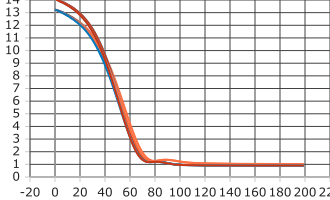
\includegraphics[width=\linewidth]{./figures/eval_MSE}%
    }%
    \hfill
    \subcaptionbox*{Mean Reciprocal Rank}[.45\linewidth]{%
        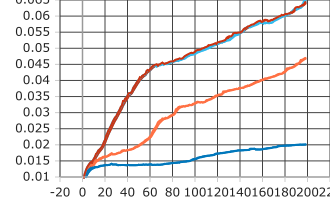
\includegraphics[width=\linewidth]{./figures/eval_Mean_Reciprocal_Rank}%
    }
    \caption{Evaluation Results}
\end{figure}

\begin{figure}[ht]
    \subcaptionbox*{Factorization Loss}[.33\linewidth]{%
        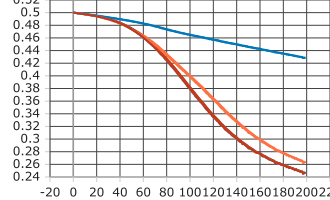
\includegraphics[width=\linewidth]{./figures/training_Factorization_Loss}%
    }
    \subcaptionbox*{Joint Loss}[.33\linewidth]{%
        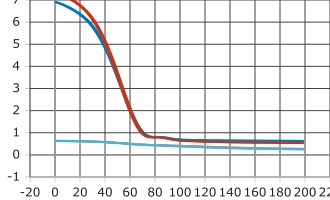
\includegraphics[width=\linewidth]{./figures/training_Joint_Loss}%
    }
    \subcaptionbox*{MSE}[.33\linewidth]{%
    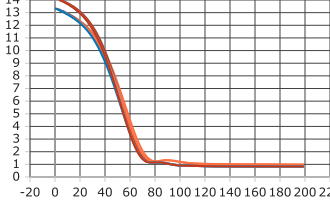
\includegraphics[width=\linewidth]{./figures/training_MSE}%
}%
    \caption{Training Results}
    \medskip
    \small
    \begin{center}
        \textcolor{orange}{Orange:} \texttt{shared=True\_LF=0.99\_LR=0.01}\\
        \textcolor{blue}{Dark Blue:} \texttt{shared=True\_LF=0.5\_LR=0.5}\\
        \textcolor{red}{Red:} \texttt{shared=False\_LF=0.5\_LR=0.5}\\
        \textcolor{cyan}{Light Blue:} \texttt{shared=False\_LF=0.99\_LR=0.01}
    \end{center}
\end{figure}


\begin{enumerate}
    \item \points{3a} Consider the case with $\lambda_F=0.99$ and $\lambda_R=0.01$. Based on the train/test loss curves, does parameter sharing outperform having separate models? 
    
    \item \points{3b} Now consider the case with $\lambda_F=0.5$ and $\lambda_R=0.5$.  Based on the train/test loss curves, does parameter sharing outperform having separate models? 
    
    \item \points{3c} In the \textbf{shared model setting} compare results for $\lambda_F=0.99$ and $\lambda_R=0.01$ and $\lambda_F=0.5$ and $\lambda_R=0.5$, can you explain the difference in performance?
\end{enumerate}